\documentclass[bachelor,nofonts]{njupthesis}

\title{这是论文题目}
\author{某某某}
\advisor{某长者}
\school{计算机学院}
\major{计算机科学与技术}
\studentclass{B150406}
\studentid{B15080000}
\graduateyear{2019}
\begindate{2019年3月11日}
\finishdate{2019年6月14日}

\begin{document}

\makecover

\begin{chineseabstract}
这是论文摘要。 

需要的话可以用多个段落。

……

\chinesekeyword{当代生活;机器学习;大咕咕咕鸡}
\end{chineseabstract}

\begin{englishabstract}
With the going on of contemporary life......



\englishkeyword{Contemporary Life;Machine Learning;Big GuGuGu Chicken}
\end{englishabstract}

\thesistableofcontents

\thesischapterexordium

\chapter{绪论}
这是正文了!

\section{研究工作的背景与意义}

当代生活\citing{pedregosa2011scikit}是严肃文学大师的作品。


\section{当代生活的国内外研究历史与现状}
字数字数字数。

\section{本文的主要贡献与创新}
本论文主要创新点与贡献如下:

\section{本论文的结构安排}
本文的章节结构安排如下:


\chapter{第二章的名字}

\section{管他叫啥}

\subsection{严肃文学}
严肃文学的具体定义如下:
\begin{equation}
c^2 = a^2 + b^2
\end{equation}

其中,$a, b, c$为三角形边的长度。

\begin{figure}[h]
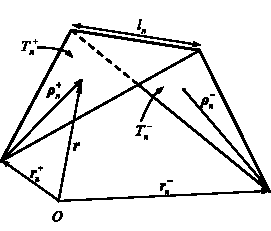
\includegraphics{pica.pdf}
\caption{我也不知道这个是什么图}
\label{pica}
\end{figure}
balabalasd



\subsection{当代文学人物}

\subsubsection{狗熊}

\subsubsection{李中猫}


\chapter{全文总结与展望}

\section{全文总结}
本文以当代生活为研究背景……

\section{后续工作展望}
严肃文学的研究近几年发展迅速,在本文研究工作的基础上,仍有以下方向值得进一步研究:

\thesisacknowledgement
本论文采用南京邮电大学本科论文\LaTeX 模版编写。


\thesisloadbibliography[nocite]{reference}

%
% Uncomment following codes to load bibliography database with native
% \bibliography command.
%
% \nocite{*}
% \bibliographystyle{njupthesis}
% \bibliography{reference}
%

\thesisappendix
这里是附录,没有请删除。

\end{document}
